\documentclass{article}
\usepackage[utf8]{inputenc}
\usepackage[T1]{fontenc}
\usepackage{lmodern}  
\usepackage{amsmath, amssymb, amsthm}
\usepackage{tikz}
\usepackage[top=2.2cm, bottom=2.5cm, left=3.5cm, right=3.5cm]{geometry}
\usepackage{caption}
\usepackage{subcaption}
\newtheorem{theorem}{Teorema}
\renewcommand{\proofname}{Demostración}
\title{Practica BFS, Dijsktra, AGM} 
\author{Nahuel}

\begin{document}
\maketitle
\section{Ejercicio 1 solucion}
\begin{theorem}
Sea $G=(V,E)$ un grafo simple y no ponderado.
Ejecutar \textbf{BFS} desde $v\in V$ produce un árbol $T$
tal que para todo $w$ alcanzable desde $v$ se cumple
\[
\operatorname{dist}_T(v,w)=\operatorname{dist}_G(v,w).
\]
En particular, $T$ es $v$-geodésico.
\end{theorem}

\begin{proof}
Denotemos por $\ell(w)$ el \emph{nivel} (número de iteración) en el que
BFS descubre a $w$.

\textbf{(i) Existe un camino de longitud $\ell(w)$ en $G$:}
BFS solo encola a $w$ cuando examina una arista $(x,w)$ con $x$ ya
extraído de la cola, y $\ell(x)=\ell(w)-1$.  Por inducción sobre
$\ell(w)$ se obtiene un camino $v\rightsquigarrow w$ con
$\ell(w)$ aristas.

\textbf{(ii) Minimalidad.}  Supongamos, hacia contradicción, que existe
un camino $P$ de $v$ a $w$ con menos de $\ell(w)$ aristas.  Sea $y$
el primer vértice de $P$ que BFS descubre \emph{después} de $v$.
Entonces su predecesor $x$ en $P$ está a nivel $<\ell(w)-1$ y la arista
$(x,y)$ haría que $y$ (o eventualmente $w$) se encolase antes,
contradiciendo la definición de $\ell(w)$.

Los incisos (i) y (ii) implican
$\ell(w)=\operatorname{dist}_G(v,w)$.
Como el camino registrado por BFS en $T$ tiene exactamente $\ell(w)$
aristas, se cumple la igualdad de distancias en el árbol;
por lo tanto $T$ es $v$-geodésico.
\end{proof}
\section*{Contraejemplo: árbol \(v\)-geodésico que no es árbol BFS}

\subsection*{Grafo \(G\)}

\begin{figure}[ht]
  \centering
  %--------- Subfigura (a): Grafo G -----------------------------
  \begin{subfigure}[t]{0.46\textwidth}
    \centering
    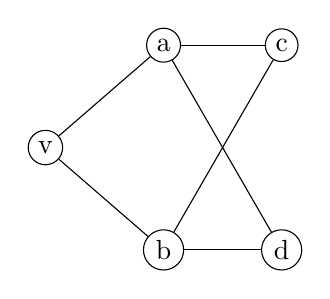
\begin{tikzpicture}[every node/.style={circle,draw,minimum size=8pt,inner sep=2pt}]
	      % Nodos grafo G
      \node (v) at (0,0)  {v};
      \node (a) at (1.5,1.3) {a};
      \node (b) at (1.5,-1.3){b};
      \node (c) at (3,1.3)  {c};
      \node (d) at (3,-1.3) {d};
      % Aristas grafo G
      \draw (v) -- (a);
      \draw (v) -- (b);
      \draw (a) -- (c);
      \draw (a) -- (d);
      \draw (b) -- (c);
      \draw (b) -- (d);
    \end{tikzpicture}
    \caption{Grafo $G$}
    \label{fig:grafoG}
  \end{subfigure}
  \hfill
  %--------- Subfigura (b): Árbol T -----------------------------
  \begin{subfigure}[t]{0.46\textwidth}
    \centering
    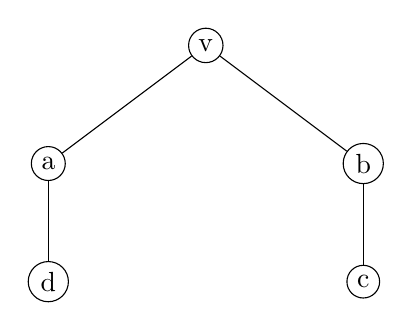
\begin{tikzpicture}[every node/.style={circle,draw,minimum size=8pt,inner sep=2pt}]
      % (mismo contenido que antes) …
      % Nodos árbol T (raíz arriba)
      \node (v) at (0,3)   {v};
      \node (a) at (-2,1.5){a};
      \node (b) at ( 2,1.5){b};
      \node (d) at (-2,0)  {d};
      \node (c) at ( 2,0)  {c};
      % Aristas árbol T
      \draw (v) -- (a);
      \draw (v) -- (b);
      \draw (a) -- (d);
      \draw (b) -- (c);
    \end{tikzpicture}
    \caption{Árbol $T=\{va, vb, ad, bc\}$}
    \label{fig:arbolT}
  \end{subfigure}
  %--------------------- Leyenda global -------------------------
  \caption{Contraejemplo: árbol $v$-geodésico que no es árbol BFS.}
  \label{fig:contraejemplo}
\end{figure} 

\begin{itemize}
  \item T es \textbf{generador} (contiene los 5 vértices y tiene 4 aristas).
  \item Las distancias en \(T\) coinciden con las de \(G\):
    \[
      \operatorname{dist}_T(v, a) = \operatorname{dist}_T(v, b) = 1, \quad
      \operatorname{dist}_T(v, c) = \operatorname{dist}_T(v, d) = 2.
    \]
\end{itemize}

Luego \(T\) es \(v\)-geodésico.

\subsection*{¿Por qué ninguna ejecución de BFS produce \(T\)?}

\begin{enumerate}
  \item Al iniciar BFS en \(v\) se encolan, en algún orden, \(a\) y \(b\).\\
        Llamemos \emph{“primero”} al que salga antes de la cola.

  \item Ese vértice primero (sea \(a\) o \(b\)) explora sus incidentes\\
        \((\text{primero}, c)\) y \((\text{primero}, d)\).\\
        Ambos vecinos están sin visitar y reciben como \emph{padre} al vértice primero; quedan encolados.

  \item Cuando salga el segundo vértice de \(\{a, b\}\),\\
        los vértices \(c\) y \(d\) ya estarán marcados,\\
        de modo que \textbf{no cambiarán de padre}.
\end{enumerate}

Así, en \textbf{todo árbol BFS} ambos vértices de nivel 2  
tienen el \textbf{mismo padre} (el que se extrajo antes entre \(a\) y \(b\)).

En el árbol \(T\) ocurre lo contrario:  
\(c\) es hijo de \(b\) y \(d\) es hijo de \(a\).  

Por lo tanto, \(T\) \textbf{no puede} obtenerse con BFS desde \(v\).

\vspace{1em}

\subsection*{En conclusión:}

\begin{itemize}
  \item Todo árbol que produce BFS es \(v\)-geodésico,

  \item pero \textbf{no todo árbol \(v\)-geodésico} puede surgir de BFS;

  \item el grafo y el árbol anteriores son un \emph{contraejemplo concreto}.
\end{itemize}

\section{Ejercicio 3 Solucion}
\begin{theorem}
Sea $G=(V,E)$ un digrafo. Sea \textbf{$H$} el digrafo bipartito construido 
de la siguiente forma:
\begin{itemize}
  \item $\forall v \in V(G)$ se crean dos copias $v^0$ y $v^1$
  \item $\forall (u,v) \in E(G)$, se agrega la arista dirigida $(u^0,v^1) \in E(H)$
\end{itemize}
Entonces, una secuencia de vertices $v_1^1, v_2^0, \dots, v_k^{k \bmod 2}$ 
es un recorrido en $H$
\end{theorem}
\noindent\textit{Nota:} Para que el enunciado tenga sentido y la equivalencia sea válida en ambos sentidos, 
asumimos que por cada arista $(v, w) \in E(G)$, el grafo $H$ contiene tanto la arista $v^0 \to w^1$ 
como la arista $v^1 \to w^0$.

\begin{proof}
  $(\Rightarrow)$ Suongamos que $v_1,v_2, \dots, v_k$ es un recorrido de $G$. Entonces
  por definicion de recorrido de un digrafo se cumple
  \[ \forall i \in \{1, \dots, k - 1\} \quad (v_i, v_{i+1}) \in E(G) \]
  Por la construccion del grafo $H$, existe una arista $(v_i^{i \bmod 2}, v_{i+1}^{i \bmod 2}) \in H $
  si y solo si $(v_i,v_{i+1}) \in E(G)$ \\ \\
  Por lo tanto: 
  \[(v_1^1,v_2^0),(v_2^0,v_3^1), \dots, (v_{k-1}^{k \bmod 2}, v_k^{k \bmod 2}) \in E(H) \] \\
  Es decir, la secuencia $v_1^1,v_2^0,v_3^1, \dots, v_k^{k \bmod 2}$ es un recorrido en $H$
\end{proof}


\end{document}
